\scanpage{106}
\mspage{105}%
i.e. que la filtration dudit foncteur a\unsure{\rlap{m}d|d}\rlap{d}met un\deleted{e} splittage compatible avec les produits tensoriels. Mais le choix d'un tel splittage équivaut à celui d'un point \deleted{sous} sur un certain torseur à droite $Q=Q'$ sous le \inserted{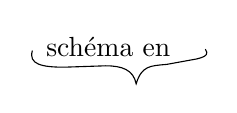
\begin{tikzpicture}[baseline=-.2ex,x=1em,y=1em]
\node[anchor=base west] at (0,.4) {schéma en};
\draw (-.15,.6) .. controls (-.3,.1) and (.2,0) .. (1,0) -- (2.5,.05) .. controls (3.1,.05) and (3.5,-.1) .. (3.6,-.6) .. controls (3.8,.05) and (4.1,.05) .. (4.7,.1) -- (5.8,.3) .. controls (6.2,.4) and (6.2,.5) .. (6.1,.65);
\end{tikzpicture}} groupes \inserted{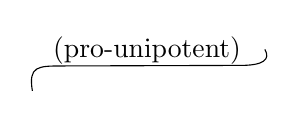
\begin{tikzpicture}[baseline=-.2ex,x=1em,y=1em]
\node[anchor=base west] at (0,.4) {(pro-unipotent)};
\draw (-.4,-.8) .. controls (-.55,.1) and (-.2,.1) .. (.7,.1) -- (7,.12) .. controls (8,.1) and (8.2,.35) .. (8,.7);
\end{tikzpicture}} $H$ des automorphismes de $F$ respectant la filtration et induisant l'identité sur le gradué associé; il n'est pas du tout canonique !

3) Appelons \uline{pré-str\rlap{c}u\rlap{u}cture de Hodge} sur un espace vectoriel \inserted{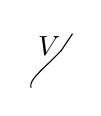
\begin{tikzpicture}[baseline=-.2ex,x=1em,y=1em]
\node[anchor=base west] at (0,.5) {$V$};
\draw (.1,-.65) .. controls (0,-.35) and (.6,.05) .. (1.2,.7) -- (1.6,1.3);
\end{tikzpicture}} de dimension finie sur $\underline{Q}$, la donnée d'une bigraduation sur $V\otimes_{\underline{Q}}\underline{C}=V_{\underline{C}}$, $V_{\underline{C}}=\handwritten{\coprod_{p,q}}V^{p,q}$, telle que a) la graduation totale correspondante soit ``définie sur $\underline{Q}$'' \uline{i.e.} $\handwritten{\coprod}_{p+q=n}V^{p,q}$ provienne d'un sous espace $V_{\underline{Q}}^n$ de $V$, et b) on a $\overset{\handwritten{\rule{.65em}{.35pt}}}{V}^{p,q}=V^{q,p}$, où $x\handwritten{\mapsto}\overset{\handwritten{\rule{.55em}{.35pt}}}{x}$ désigne la conjuguaison complexe. \unsure{(}NB Généralisation à des corps plus généraux laissée à Saavedra). Les vectoriels $V$ munis d'une pré-structure de Hodge forment une catégorie tensorielle sur $\underline{Q}$ dans un sens évident, muni d'un foncteur fibre canonique, le foncteur ``oubli''\inserted{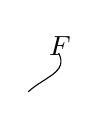
\begin{tikzpicture}[baseline=-.2ex,x=1em,y=1em]
\node[anchor=base west] at (0,.4) {$F$};
\draw (.7,.5) .. controls (1.05,-.2) and (.2,-.35) .. (-.4,-.9);
\end{tikzpicture}}. On trouve donc un groupe de \unsure{$\mathbb{G}$|G}alois $G$, et \deleted{tout} plus généralement toute \inserted{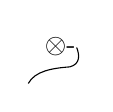
\begin{tikzpicture}[baseline=-.2ex,x=1em,y=1em]
\node[anchor=base west] at (0,.4) {$\otimes$-};
\draw (-.25,-.7) .. controls (0,-.25) and (.6,-.15) .. (1.25,-.1) .. controls (1.65,0) and (1.6,.35) .. (1.5,.6);
\end{tikzpicture}}sous-catégorie $\underline{C}$ de la catégorie précédente nous définit un groupe de Galois $G$. La bigraduation sur le foncteur \deleted{oubli} $F_{\underline{C}}(V)=V\otimes_{\underline{Q}}\underline{C}$ correspond, en vertu de 1) (où il convient cependant de se permettre une extension du corps de base sur le foncteur fibre envisagé ....) d'un homomorphisme ${\underline{G}_m}_{\underline{C}}^2\handwritten{\longrightarrow}G_{\underline{C}}$, i.e. de deux homomorphismes \inserted{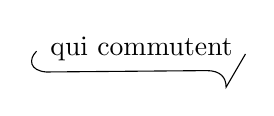
\begin{tikzpicture}[baseline=-.2ex,x=1em,y=1em]
\node[anchor=base west] at (0,.5) {qui commutent};
\draw (-.15,.65) .. controls (-.45,.35) and (-.4,-.05) .. (.2,-.1) -- (6,-.05) .. controls (6.5,-.05) and (6.7,-.3) .. (6.7,-.65) -- (7.4,.55);
\end{tikzpicture}}
\[
i_1,i_2:{\underline{G}_m}_{\underline{C}}\handwritten{\longrightarrow}G_{\underline{C}}.
\]
Les deux conditions a) et b) imposées aux structures envisagées s'interprètent respectivement par les faits que l'homomorphisme
\[
i_{\underline{C}}=i_1i_2\unsure{\doteqdot|=}\handwritten{\lambda\mapsto}i_1(\handwritten{\lambda})i_2(\handwritten{\lambda})
\]
est ``défini sur $\underline{Q}$'' i.e. provient d'un homomorphisme
\[
i:\underline{G}_m\handwritten{\longrightarrow}G,
\]
\margin{\tikz[baseline=0pt,x=1em,y=1em]{\draw (0,0) .. controls (.1,.05) and (.17,.15) .. (.22,.3);}}(nécessairement central, car les composantes homogènes $V_{\underline{Q}}^n$ d'une pré-structure de Hodge sont \deleted{nécessairement}\inserted{évidemment} munis d'une \inserted{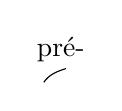
\begin{tikzpicture}[baseline=-.2ex,x=1em,y=1em]
\node[anchor=base west] at (0,.4) {pré-};
\draw (.6,-.55) .. controls (.8,-.25) and (1.1,-.15) .. (1.4,-.05);
\end{tikzpicture}}structure de Hodge de façon que $V$ soit la somme directe de $V_{\underline{Q}}^n$ en tant que pré-structure

